\chapter*{Appendix A}
\addcontentsline{toc}{chapter}{Appendix A}
\label{appA}

$$f_1 = (x - p_x)^{n+1} - (y - p_y)^2 - (z - p_z)^2$$
$$f_2 = - x - q$$
$$f_3 = f_1 \cap f_2$$
$$f_3 = f_1+f_2-\sqrt{f_1^2+f_2^2}$$
$$f_4 = x + q + q \cdot cos\left(k \sqrt{(y - p_y)^2 + (z - p_z)^2}\right)$$
$$f_5 = 4 h^{n+1} - (z - p_z)^2 - (y - p_y)^2$$
$$f_6 = f_4 \cap f_5$$
$$f_6 = f_4+f_5-\sqrt{f_4^2+f_5^2}$$
$$f_7 = x$$
$$f_8 = f_6 \cup f_7$$
$$f_8 = f_6 + f_7 + \sqrt{f_6^2+f_7^2}$$
$$f_9 = x+q$$
$$f_{10} = f_8 \cap f_9$$
$$f_{10} = f_8 + f_9 - \sqrt{f_8^2+f_9^2}$$
$$f_{11} = f_{10} \cup f_3$$
$$f_{11} = f_{10} + f_3 + \sqrt{f_{10}^2+f_3^2}$$
$$f_{11} = $$

The corresponding surfaces are displayed on the figure \ref{img:27}
\begin{figure}
    \centerline{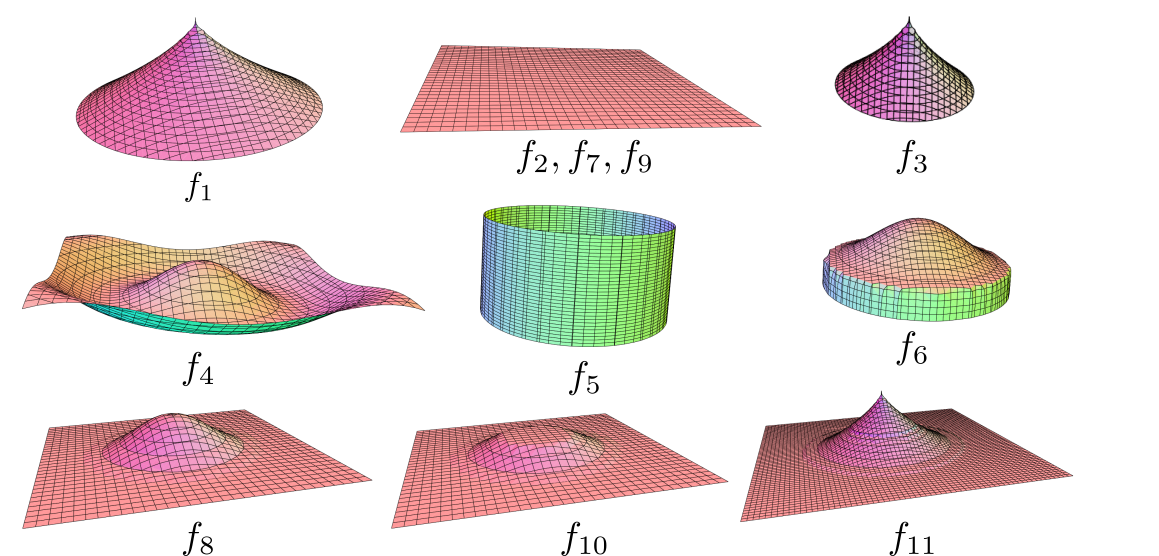
\includegraphics[scale=0.5]{images/img27}}
    \caption[Attaching the singularity to a plane using CSG]
    {Attaching the singularity to a plane using CSG.}
    %id obrazku, pomocou ktoreho sa budeme na obrazok odvolavat
    \label{img:27}
\end{figure}